\section{Feature engineering}

Before we can apply the algorithms covered in class to tackle this problem, we need to understand and organize the data being used.

\subsection{Description of the Data}

Firstly, the training data consists of approximately 296,000 rows and exactly 45 columns. Among these 45 columns, they are:

\begin{itemize}
    \item The \textbf{Polygon} that corresponds to the geographical area under study. Polygons are described as a list of points.
    \item The \textbf{Urban type}. It describes the urban characteristics of the photo. There are six types of urban landscapes: Dense Urban, Industrial, Rural, Sparse Urban, Urban Slum, and N/A. A location may belong to multiple categories simultaneously.
    \item The \textbf{Geography type}. It describes the characteristics of the environment of the photo. There are 12 types of geography type: Barren Land, Coastal, Dense Forest, Desert, Farms, Grass Land, Hills, Lakes, River, Snow, Sparse Forest, and N/A. A location may also belong to multiple categories.
    \item For each photo, the \textbf{Dates of the picture} in the 'dd-mm-yyyy' format.
    \item For each photo, the \textbf{Average and the Standard deviation of primary colors} (red, green, blue) in the picture.
    \item For each photo, the \textbf{Change status} for each photo. It describes the recent event that happened in the photo. There are ten types of them: Materials Introduced, Construction Done, Land Cleared, Construction Midway, Prior Construction, Construction Started, Materials Dumped, Greenland, Operational, and Excavation.
\end{itemize}

Moreover, only the training data contains labels in the \textbf{Change type} column. Below is the histogram showing the frequency of each category of labels. It is interesting to notice are not equally distributed.

\begin{center}
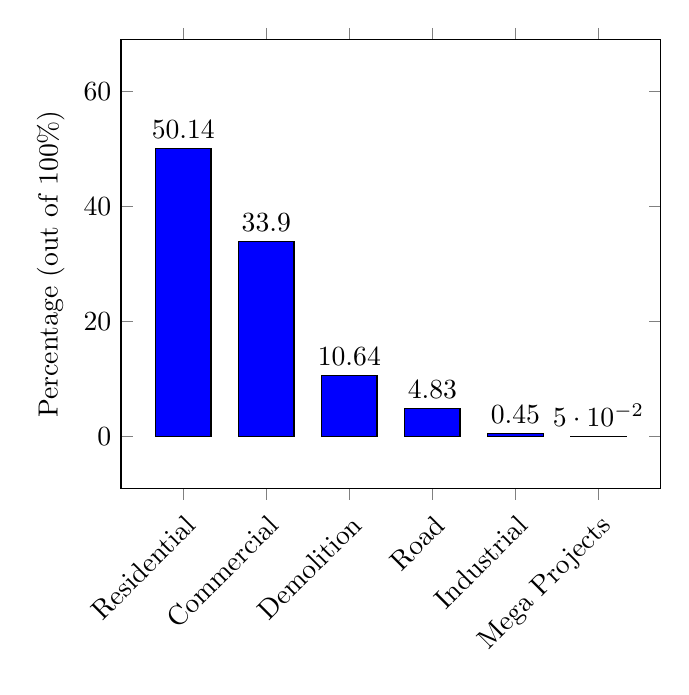
\begin{tikzpicture}
\begin{axis}[
    symbolic x coords={Residential, Commercial, Demolition, Road, Industrial, Mega Projects},
    ylabel = {Percentage (out of 100\%)},
    xlabel = {},
    xtick=data,
    xticklabel style={rotate=45,anchor=north east},
    nodes near coords,
    nodes near coords align={vertical},
    ymin=0,
    ymax=60,
    ybar,
    bar width=20pt,
    enlargelimits=0.15,
    ]
    \addplot[fill=blue] coordinates {
        (Residential, 50.14)
        (Commercial, 33.90)
        (Demolition, 10.64)
        (Road, 4.83)
        (Industrial, 0.45)
        (Mega Projects, 0.05)
    };
\end{axis}
\label{histo}
\end{tikzpicture}
\end{center}

\subsection{Dealing with missing data}

Firstly, it was necessary to address the missing data. Indeed, the majority of algorithms studied in class and used in Machine Learning operate on complete data rather than columns with missing data. Some columns are unaffected by this phenomenon, such as Urban type, Geography type, and Geometry. However, all other columns have missing data, typically ranging from 1383 to 1954 missing entries. \\ \\
Upon closer analysis of the missing data for each geographical type, it was noted that the number of missing entries was negligible compared to the total sample size. The initial instinct was to remove the rows with missing data. However, this approach was not feasible as we needed to be able to predict a geographical type for any input data format.\\ \\
Therefore, we opted to replace the missing data with the mean for each numerical column and the mode for categorical data. This method of replacement with the mean and mode allows us to populate the table, albeit with potentially inaccurate information. Nevertheless, this approach is unlikely to significantly impact the results given the negligible frequency of missing data and the use of common replacement values.

\subsection{Sorting columns in chronological order}

The dates were not sorted. For example, date 1 could correspond to November 28, 2019, and date 2 to December 13, 2013. Therefore, they needed to be arranged in chronological order. To achieve this, we utilized sorting with the Datetime format of the \texttt{Pandas} module. Consequently, for each feature associated with a date, it was necessary to reorder them chronologically according to their respective rows.\\ \\
Rather than considering the dates themselves as data for our model, we chose to focus solely on the time interval between each date. This approach makes more sense because a date without reference is meaningless, and furthermore, the information in the Change Status column is very likely to depend on the time difference from the previous date.\\ \\
We also included the mean and standard deviation of each primary color in our data. Of course, since these numerical data are always between 0 and 255, we standardized them.

\subsection{Encoding categorical columns}

Afterwards, it was necessary to process the categorical data. Only the columns 'Geography Type', 'Urban type', and 'Change status' for each date were in this form. The initial idea was to apply one-hot encoding for these data. This is precisely what we did for 'Geography Type' and 'Urban type'. This approach is entirely suitable since these data can belong to multiple types, and these columns appear only once for each photo. \\ \\
However, this idea is quite ineffective with the 'Change status' columns. Each 'Change Status' belongs to a single category among the 10 existing ones. Also, there are 5 'Change status' columns for the 5 existing dates. This means that if we had applied one-hot encoding, it would have resulted in 50 columns. For these two reasons, we preferred to establish a correspondence between each category and an integer between 0 and 9, inclusive. This saved us 45 columns and is much more efficient. Also, by analyzing the construction features, we realize that they follow a chronological order. Therefore, we classified the numbers from 0 to 9 according to the chronological order.

\subsection{Creating new features}

We also created a new feature. For example, for the polygons, we considered the area of each polygon, but we also took into account the convexity of the shape. To achieve this, the selected feature is the ratio between the area of the polygon and the area of its convex hull. This results in a number between 0 and 1. The closer this number is to 1, the more convex the polygon is. After analysis, it was found that 17,069 (or 15\%) of the surfaces are non-convex. This is coherent because a road is likely to be convex, but a building is not necessarily so. Therefore, this indicator is relevant for our problem.

\subsection{Treating large-scale Data}

As we have large-scale data, we chose to save this data in multiple files to avoid recalculating them for each test of our model. For this purpose, we used the 'Save' function of the \texttt{NumPy} module.\\ \\
Next, the last thing we did was to reduce the dimensionality of the data to reduce computation time and potentially increase the efficiency of our model. For this, we performed Principal Component Analysis (PCA). We retained the minimum number of dimensions to preserve 85\% of the energy of our original data.
